\documentclass[12pt, a4paper]{article}
\usepackage[a4paper, top=2.5cm, bottom=2.5cm, left=2.5cm, right=2.5cm]{geometry}
\usepackage[spanish]{babel}
\usepackage[utf8x]{inputenc}
\usepackage{multirow} % para las tablas
\usepackage{graphicx} % para las imagenes
\usepackage{fancyhdr} % para estilo cabeceras y pies de página
\usepackage{hyperref} % para los hyperlinks entre secciones
\usepackage{float}
\usepackage{array}
\usepackage{booktabs}

\pagestyle{fancy} % seleccionamos un estilo
\lhead{Grupo 1.1} % texto izquierda de la cabecera
\chead{Bases de datos avanzadas} % texto centro de la cabecera
\rhead{TGR} % texto derecha de la cabecera

\rfoot{Página \thepage \hspace{1mm}  de \pageref{LastPage}} % texto derecha del pie de página
\renewcommand{\headrulewidth}{0.4pt} % grosor de la línea de la cabecera
\renewcommand{\footrulewidth}{0.4pt} % grosor de la línea de la cabecera

\begin{document}
	\newpage
	
	\begin{titlepage} % Logo empresa

		\begin{figure}[h]
			\centering
			
\includegraphics[width=10cm]{Imagenes/logo-udc}
		\end{figure}
	
		\begin{center}
			% Nombre empresa
			\LARGE{\textbf{Bases de datos avanzadas}}
			\\[0.5cm]
			
			% Nombre documento
			\Large{\textbf{TGR - Aplicación en Pro*C}}
			\\[2cm]
			
			% Autor
			\Large Elías García Mariño
			\\[0.5cm]
			\Large elias.garcia@udc.es
			\\[0.5cm]
			\Large 35489113K
			\\[2cm]
			
			% Fecha
			\Large Mayo 17, 2016
		\end{center}
	
	\end{titlepage}
	
	\newpage
	\tableofcontents
	
	\newpage
	\section{Introducción}
	El objetivo de este documento es proporcionar una visión detallada de la base de datos planteada para la realización de este TGR. \\\par
	Se plantea entonces, una base de datos sencilla para una pequeña empresa dedicada al sector del fitness, la cual cuenta con varios monitores que asesorarán a los clientes, creando planes de entrenamiento adecuados a las necesidades de cada uno.
	
	\section{Aclaraciones}
	\begin{itemize}
		\item Las restricciones de integridad de clave primaria y clave foránea de una entidad se detallan en la tabla del diccionario de datos correspondiente a dicha entidad.
		\item Las restricciones de integridad de cualquier otro tipo se detallarán en una subsección dedicada íntegramente a ellas dentro de la sección correspondiente a dicha entidad en el diccionario de datos. 
	\end{itemize}
	\section{Diagrama entidad relación}
		\begin{figure}[h]
			\centering
			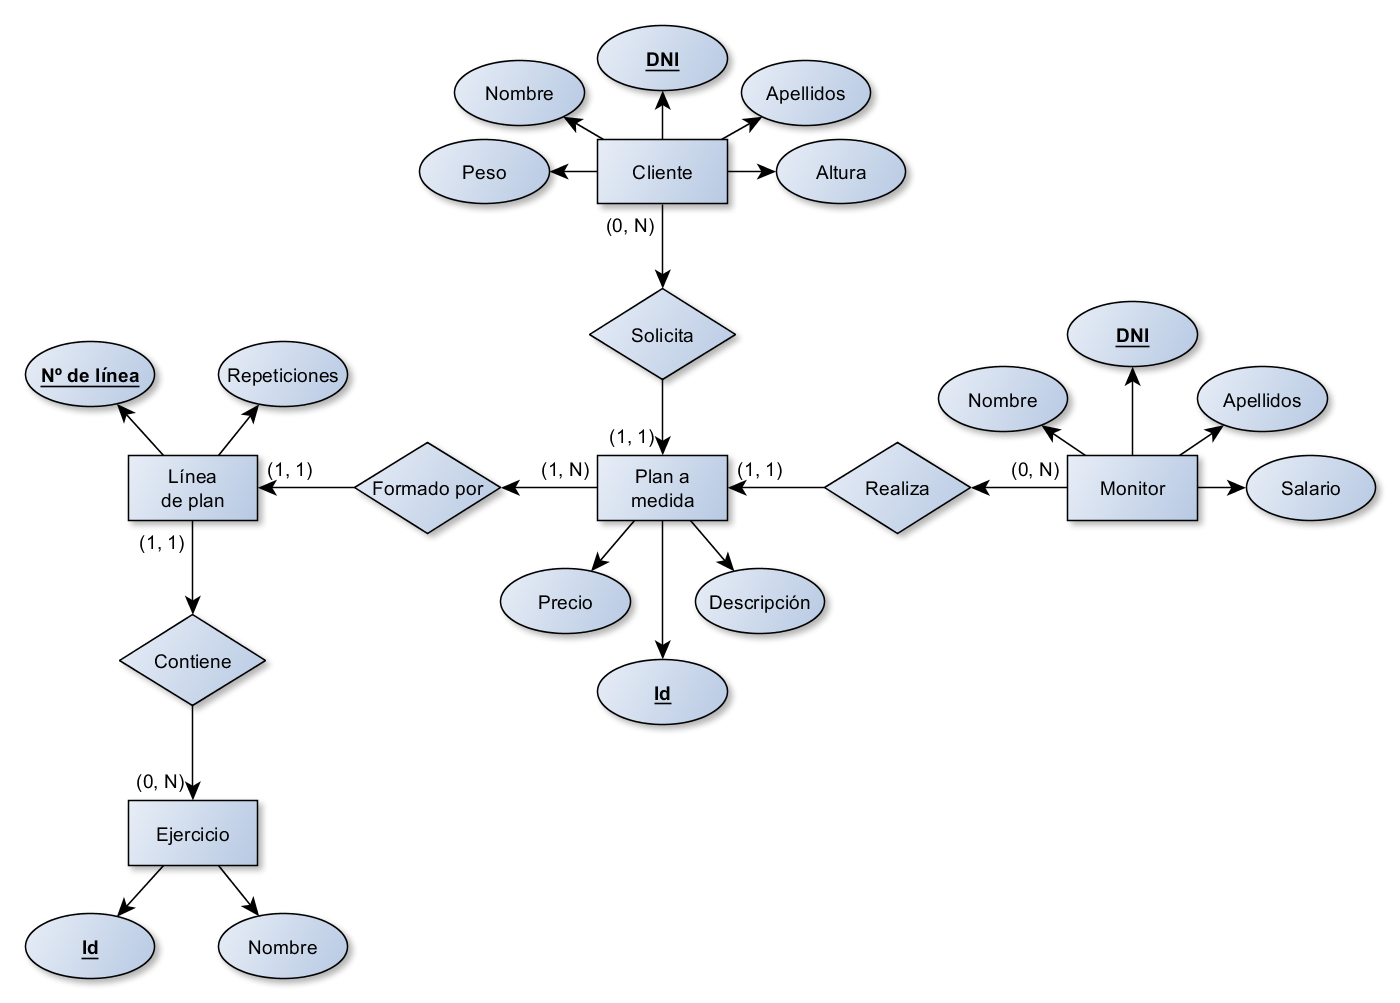
\includegraphics[width=16cm]{Imagenes/entidad_relacion}
		\end{figure}
	
	\newpage
	\section{Modelo relacional}
	\begin{figure}[h]
		\centering
		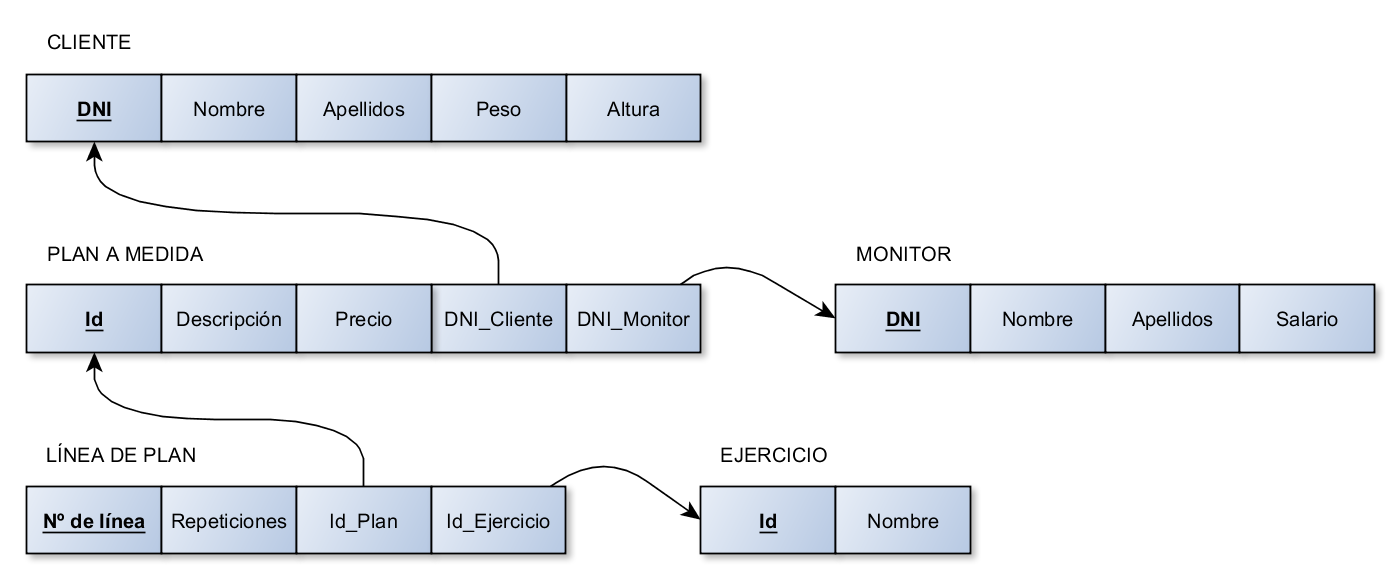
\includegraphics[width=16cm]{Imagenes/modelo_relacional}
	\end{figure}
	
	\section{Diccionario de datos}
	
	\subsection{Cliente}
	\subsubsection*{Descripción}
	Entidad que almacena los datos de los clientes, los cuales se registran al solicitar un plan de entrenamiento personalizado y tras haber realizado un pesaje y una medición previa.
	\subsubsection*{Restricciones de integridad}
	En esta entidad, además de la clave primaria, se ha incluido una restricción de CHECK sobre el atributo \textbf{DNI}, la cual comprueba que el DNI a insertar contenga ocho dígitos seguidos de una letra mayúscula.
	\subsubsection*{Relaciones}
	La entidad \textbf{Cliente} tiene una relación 0:N con \textbf{Plan}.
	\begin{table}[H]
		\centering
		\caption{Atributos Cliente}
		\begin{tabular}{@{} m{2.5cm} m{5.5cm} m{7cm} @{}}
			\toprule
			\textbf{Campo} & \textbf{Tipo} & \textbf{Descripción} \\ \midrule
			\underline{DNI} & VARCHAR(9) NOT NULL & DNI del cliente. Es la clave primaria. \\
			Nombre & VARCHAR2(15) NOT NULL & Nombre del cliente. \\	
			Apellidos & VARCHAR2(40) NOT NULL & Apellidos del cliente \\
			Peso & NUMBER(5,2) NOT NULL & Peso del cliente. \\	
			Altura & NUMBER(3,2) NOT NULL & Altura del cliente. \\ \bottomrule
		\end{tabular}
	\end{table}
	
	\newpage
	\subsection{Monitor}
	\subsubsection*{Descripción}
	Entidad que almacena los datos de los monitores contratados por la empresa, los cuales se encargarán de crear y supervisar planes personalizados solicitados para los clientes.
	\subsubsection*{Restricciones de integridad}
	En esta entidad, además de la clave primaria, se ha incluido una restricción de CHECK sobre el atributo \textbf{DNI}, la cual comprueba que el DNI a insertar contenga ocho dígitos seguidos de una letra mayúscula.
	\subsubsection*{Relaciones}
	La entidad \textbf{Monitor} tiene una relación 0:N con \textbf{Plan}.
	\begin{table}[H]
		\centering
		\caption{Atributos Monitor}
		\begin{tabular}{@{} m{2.5cm} m{5.5cm} m{7cm} @{}}
			\toprule
			\textbf{CAMPO} & \textbf{TIPO} & \textbf{DESCRIPCIÓN} \\ \midrule
			\underline{DNI} & VARCHAR(9) NOT NULL & DNI del monitor. Es la clave primaria. \\
			Nombre & VARCHAR2(15) NOT NULL & Nombre del monitor. \\
			Apellidos & VARCHAR2(40) NOT NULL & Apellidos del monitor. \\
			Salario & NUMBER(8,2) NOT NULL & Salario del monitor. \\ \bottomrule
		\end{tabular}
	\end{table}
	
	\subsection{Plan a medida}
	\subsubsection*{Descripción}
	Entidad que almacena los datos administrativos de los planes de entrenamiento personalizados, como una breve descripción y el precio total que tendrá que abonar el cliente.
	\subsubsection*{Relaciones}
	La entidad \textbf{Plan} tiene una relación 1:1 con \textbf{Cliente} y \textbf{Monitor} y 1:N con \textbf{Línea de plan}.
	\begin{table}[H]
		\centering
		\caption{Atributos Plan a medida}
		\begin{tabular}{@{} m{2.5cm} m{5.5cm} m{7cm} @{}}
			\toprule
			\textbf{CAMPO} & \textbf{TIPO} & \textbf{DESCRIPCIÓN} \\ \midrule
			\underline{Id} & NUMBER(10) NOT NULL & Identificador del plan a medida. Es la clave primaria. \\
			Descripción & VARCHAR2(40) NOT NULL & Breve descripción del plan. \\	
			Precio & VARCHAR2(40) NOT NULL & Precio total del plan. \\
			Cliente\textunderscore DNI & NUMBER(8,2) NOT NULL & DNI del cliente solicitante del plan. Clave foránea que referencia a la tabla \textbf{Cliente}. \\	
			Monitor\textunderscore DNI & NUMBER(8,2) NOT NULL & DNI del monitor encargado de crear y supervisar el plan. Clave foránea que referencia a la tabla \textbf{Monitor}. \\ \bottomrule
		\end{tabular}
	\end{table}
	
	\newpage
	\subsection{Ejercicio}
	\subsubsection*{Descripción}
	Entidad que almacena todos los ejercicios disponibles para emplear en los planes de entrenamiento personalizados.
	\subsubsection*{Relaciones}
	La entidad \textbf{Ejercicio} tiene una relación 0:N con \textbf{Línea de plan}.
	\begin{table}[H]
		\centering
		\caption{Atributos Ejercicio}
		\begin{tabular}{@{} m{2.5cm} m{5.5cm} m{7cm} @{}}
			\toprule
			\textbf{CAMPO} & \textbf{TIPO} & \textbf{DESCRIPCIÓN} \\ \midrule
			\underline{Id} & NUMBER(10) NOT NULL & Identificador del ejercicio. Es la clave primaria. \\ 
			Nombre & VARCHAR2(30) NOT NULL & Nombre del ejercicio. \\ \bottomrule
		\end{tabular}
	\end{table}
	
	\subsection{Línea de plan}
	\subsubsection*{Descripción}
	Entidad que almacena los ejercicios incluidos en cada plan, así como el número de veces que el cliente tendrá que repetir cada ejercicio.
	\subsubsection*{Relaciones}
	La entidad \textbf{Línea de plan} tiene una relación 1:1 con \textbf{Ejercicio} y \textbf{Plan a medida}.
	\begin{table}[H]
		\centering
		\caption{Atributos Línea de plan}
		\begin{tabular}{@{} m{2.5cm} m{5.5cm} m{7cm} @{}}
			\toprule
			\textbf{CAMPO} & \textbf{TIPO} & \textbf{DESCRIPCIÓN} \\ \midrule
			\underline{Numero\textunderscore linea} & NUMBER(10) NOT NULL & Identificador de la línea del plan. Es la clave primaria. \\
			Repeticiones & NUMBER(4) NOT NULL & Número de veces que se debe repetir cada ejercicio del plan. \\
			Plan\textunderscore Id & NUMBER(10) NOT NULL & Id del plan. Clave foránea que referencia a la tabla \textbf{Plan}. \\
			Ejercicio\textunderscore Id & NUMBER(10) NOT NULL & Id del ejercicio. Clave foránea que referencia a la tabla \textbf{Ejercicio}. \\ \bottomrule
		\end{tabular}
	\end{table}

	\section{Datos almacenados en las tablas}
	\begin{table}[H]
		\caption{Cliente}
		\centering
		\begin{tabular}{@{} m{0.5cm} m{2.2cm} m{2.4cm} m{5cm} m{1.4cm} m{2cm} @{}}
			\toprule
			\textbf{ID} & \textbf{DNI} & \textbf{NOMBRE} & \textbf{APELLIDOS} & \textbf{PESO} & \textbf{ALTURA} \\ \midrule
			1           & 43266653L    & PABLO           & MANZANARES GARCIA  & 80            & 1.79            \\
			2           & 60590504V    & JORGE           & CODINA RODA        & 74            & 1.82            \\
			3           & 61061730L    & DANIEL          & PRESA MENDIZABAL   & 93            & 1.90            \\ \bottomrule
		\end{tabular}
		\par
	\end{table}
	\begin{table}[H]
		\centering
		\caption{Monitor}
		\begin{tabular}{@{} m{0.5cm} m{2.2cm} m{2.4cm} m{5cm} m{4cm} @{}}
			\toprule
			\textbf{ID} & \textbf{DNI} & \textbf{NOMBRE} & \textbf{APELLIDOS} & \textbf{SALARIO} \\ \midrule
			1           & 50444584H    & EMILIO          & DIEGUEZ FARINA     & 1500             \\
			2           & 39317485C    & ALVARO          & PAZOS CARRACEDO    & 1300            \\ \bottomrule
		\end{tabular}
	\end{table}
	\begin{table}[H]
		\centering
		\caption{Plan}
		\begin{tabular}{@{} m{0.5cm} m{4.5cm} m{2cm} m{3.5cm} m{3.5cm} @{}}
			\toprule
			\textbf{ID} & \textbf{DESCRIPCION}  & \textbf{PRECIO} & \textbf{CLIENTE\_DNI} & \textbf{MONITOR\_DNI} \\ \midrule
			1           & PLAN DE CALENTAMIENTO & 150             & 43266653L             & 50444584H             \\
			2           & PLAN DE FUERZA        & 230             & 43266653L             & 39317485C             \\
			3           & PLAN DE FUERZA        & 230             & 61061730L             & 39317485C             \\ \bottomrule
		\end{tabular}
	\end{table}	
	\begin{table}[H]
		\centering
		\caption{Ejercicio}
		\begin{tabular}{@{} m{0.5cm} m{14.5cm} @{}}
			\toprule
			\textbf{ID} & \textbf{NOMBRE}                \\ \midrule
			1           & CUELLO-NEGACION                \\
			2           & ROTACION DE CADERA             \\
			3           & ESTIRAMIENTO LATERAL DE HOMBRO \\
			4           & ELEVACION DE HOMBROS ALTERNO   \\
			5           & PRESS DE PECHO                 \\
			6           & CURL DE BICEPS                 \\
			7           & PRESS DE PIERNA                \\ \bottomrule
		\end{tabular}
	\end{table}
	\begin{table}[H]
		\centering
		\caption{Línea}
		\begin{tabular}{@{}m{4cm} m{4.cm} m{2.4cm} m{3.6cm}@{}}
			\toprule
			\textbf{NUMERO\_LINEA} & \textbf{REPETICIONES} & \textbf{PLAN\_ID} & \textbf{EJERCICIO\_ID} \\ \midrule
			1                      & 20                    & 1                 & 1                      \\
			2                      & 20                    & 1                 & 2                      \\
			3                      & 20                    & 1                 & 3                      \\
			4                      & 20                    & 1                 & 4                      \\
			5                      & 10                    & 2                 & 5                      \\
			6                      & 10                    & 2                 & 6                      \\
			7                      & 10                    & 2                 & 7                      \\
			8                      & 10                    & 3                 & 5                      \\
			9                      & 10                    & 3                 & 6                      \\
			10                     & 10                    & 3                 & 7                      \\ \bottomrule
		\end{tabular}
	\end{table}
	
	\section{Restricciones en la implementación}
	\begin{itemize}
		\item Todas las tablas excepto \textbf{Cliente} y \textbf{Monitor} tienen un identificador generado automáticamente mediante una secuencia. Antes de la inserción de una nueva fila en una de estas tablas, un trigger se encargará de asignar un valor único a partir de la secuencia a la nueva fila. Las secuencias nos garantizan la correcta concurrencia, ya que son locales a cada sesión.
		\item Aunque en la aplicación desarrollada no se necesita, se ha utilizado una política de borrado ON DELETE CASCADE para todas las tablas con clave foránea, que, de ser necesario en un futuro, nos ahorraría tiempo al no tener que realizar nosotros una implementación de una política de borrado de claves foráneas.
		\item Anteriormente se han comentado las restricciones de CHECK en las entidades \textbf{Cliente} y \textbf{Monitor}. Dichas restricciones solo comprueban mediante un regex que el formato introducido es de ocho dígitos seguidos de una letra mayúscula. Cabe especificar que el usuario puede introducir una letra tanto mayúscula como minúscula, para otorgar de mayor flexibilidad a la aplicación. Ésta, se encargará de convertir el valor introducido por el usuario a uno compatible con la tabla sobre la que se vaya a insertar, en este caso, convirtiendo la letra a mayúscula.
		\item En la tabla \textbf{Línea} se declara una restricción UNIQUE de las columnas plan\textunderscore id y ejercicio\textunderscore id, de forma que no se puede repetir un ejercicio en un mismo plan personalizado.
		\item Respecto a la transaccionalidad, se utiliza siempre el nivel de aislamiento por defecto de Oracle, READ-COMMITED, excepto para las actualizaciones, que se utiliza SERIALIZABLE. Siempre se efectúa un COMMIT si la transacción ha sido realizada sin errores, y en el caso contrario se especifica cual ha sido el error y se realiza un ROLLBACK. Con las funcionalidades implementadas en la aplicación, no es necesario el uso de SAVEPOINTS.
	\end{itemize}
	\label{LastPage} % Referencia para obtener el numero total de páginas
	
\end{document}